\documentclass[a4paper,10pt]{article}
\usepackage[utf8]{inputenc}
\usepackage{xspace}
\usepackage{graphicx,graphics} 
\usepackage{hyperref} 
\usepackage{mathtools, bm}
\usepackage{amssymb, bm}

\usepackage{algorithm2e}
\SetAlgoLined
\SetKwProg{MyStruct}{Struct}{ contains}{end}



\graphicspath{{img/}}

%opening
\title{Algorithmic model for N-GREEN optical ring}




\begin{document}

\maketitle
\section{Introduction}
Blabla sur le contexte du projet NGREEN



\section{Model}
  \label{model}
  \subsection{Optical ring}
  Consider a directed circular graph $C_N$ representing an optical ring. $N$ is the number of nodes on the ring/the graph. Each arc $(u,v)$ is labeled by an integer distance $d(u,v)$ corresponding to the physical delay of the link in the ring, i.e. the time taken by a signal to go from $u$ to $v$ using this arc.
  
  \subsection{Message Granularity}
    The time is discretized. The unit of time is the {\bf time slot}. Each arc $(u,v)$ can be represented as a sequence of {\bf slots} $\{s_1, ... , s_k\}$, with $k = d(u,v)$. We denote by $s_n(u,v)$ the $n^{th}$ slot of the arc $(u,v)$. $s_i(v), i\in \{-d(u,v), ... , -1\} \cup \{1 , ... , d(v,w)\}$ is the $i^{th}$ slot after (before if $i<0$) v on the ring.
    On the following example, the red slot can be denoted by $s_2(u,v)$, $s_2(u)$ or $s_{-6}(v)$. 
    \begin{figure}[h]
    \centering
      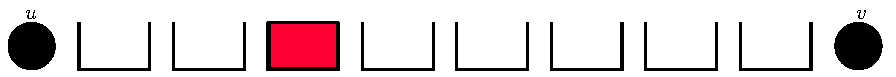
\includegraphics[scale=0.5]{suv.pdf}

      \caption{A link $(u,v)$ represented as a sequence of slots}
  \end{figure}
  
  Each node $v$ has a reading access on $s_{-1}(v)$ and a writing access on $s_{1}(v)$. Those slots are named respectively the reading and writing slots of $v$. Thus, during a time slot, a node $v$ can insert a {\bf packet} on it's writing slot, if it is allowed to. We will define the right of the nodes later on this paper. Then, at the end of the time slot, each packets skip to the next slot. A packet emitted by a node $u$ on it's writing slot $s_1(u)$ will be available in reading for a node $v$ on it's reading slot $s_{-1}(v)$ $d(u,v) -1$  time slot later.
\begin{figure}[h!]
      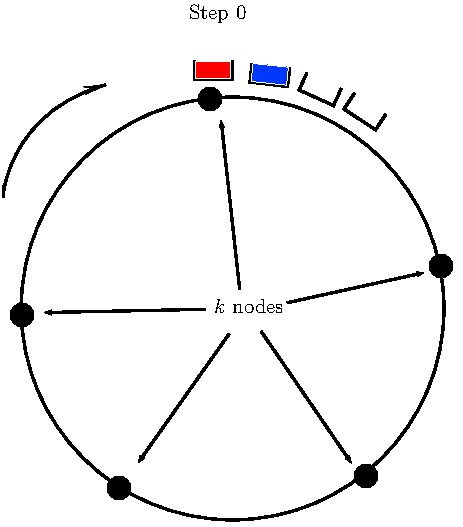
\includegraphics[scale=0.5]{anneau1.pdf}
      \hspace{3cm}
      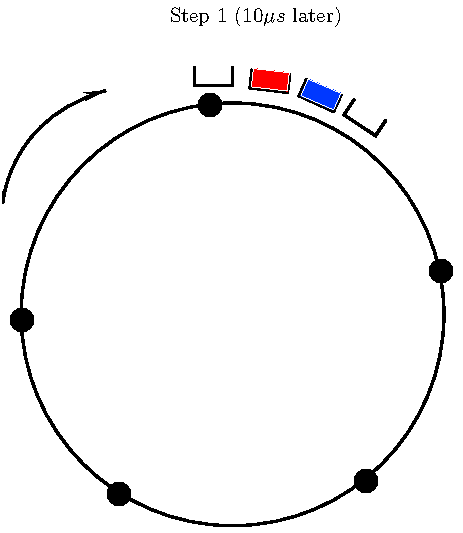
\includegraphics[scale=0.5]{anneau2.pdf}
      \caption{One rotation of the ring}
  \end{figure}
  \subsection{Broadcast and select policy}
  The ring follows a broadcast and select behavior. When a packet is inserted in a slot on the ring, by a node, no other nodes are able to write on this slot. This packets can contain some data from several nodes on the ring, that are able to read in the packet. The only node which has the right to remove the packet from the slot is the owner. This mean that every packet makes exactly one lap of the ring. Furthermore, to write on a slot, a node has to have an empty slot in it's writing slot.
  
    \subsection{CRAN Context}
    Our study takes place in the C-RAN context. The purpose is to centralise the calculation units of some antennas, distributed on the field. To each antenna, called RRH (Remote Radio Head), is associated a BBU (BaseBand Unit) in the datacenter.
      The periodic process is the following: each {\bf period $P$}, every RRH send some datas thought the ring to it's BBU, then, after a computation time in the BBU, this latter answers to the corresponding RRH. 
      The time between the emission of the message by the RRH and the reception of the answers by the same RRH is called {\bf process time} and must not be too large, considering some 5G standards.
      In this paper we will consider that all the BBU are grouped in the same node, called {\bf datacenter}, and that the antennas are distributed on the others node of the ring.
  
  
    
  \subsection{Into the node : Two kind of traffics}
    To build the packets that are sent in the ring, the nodes have to deal with two kinds of traffic: 
    \begin{itemize}
    \item The {\bf Best effort traffic}, representing the internet flow.
    \item The {\bf C-RAN traffic}, representing the high priority flow.
    \end{itemize}
    Let us denote {\bf BE-message} and {\bf CRAN-message} the unit of data of this flows. A packet is made of several BE-messages or CRAN-messages, and can be a combination of both kind of messages.
    The messages coming to a node are buffered, and the nodes send a packet with the messages if : 
     \begin{itemize}
    \item The oldest message has arrived on the buffer before $t - \alpha$, if  $t$ is the actual time.
    \item The fill rate of the buffer is greater or equal than $\beta$.
    \end{itemize}
    Those parameters $\alpha$ and $\beta$ are fixed by the network specification.

    \begin{figure}[h!]
        \begin{center}
      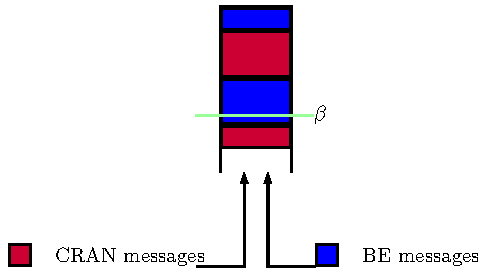
\includegraphics[scale=0.5]{insertionbuff.pdf}

      \caption{The packet creation buffer}
      \end{center}
  \end{figure}

This behavior is the basic one, the buffer of a node is filled following the FIFO rule by the BE and C-RAN traffics. Then, when the node has an available free slot, the packet is created and inserted in the slot if one of the previous constraints are satisfied. Otherwise the node does not send anything in the ring and wait for the next free slot.

    \begin{figure}[h!]
\begin{center}   

      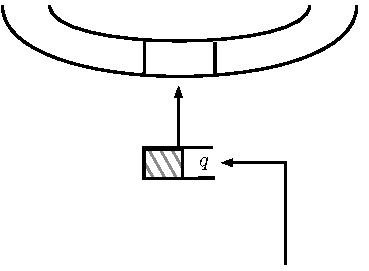
\includegraphics[scale=0.7]{insertion0.pdf}

     \caption{No management mode.}
\end{center}
  \end{figure}
  
  In order to improve the CRAN-messages latency, we first imagined the following solution. Each nodes have two buffers. One for the BE-messages, and one fore the CRAN-messages. When a node is able to send some messages on the ring, i.e. the slot on it's writing slot is free, the packet is filled with the CRAN-messages first. 
  
  
    \begin{figure}[h!]
\begin{center}   

      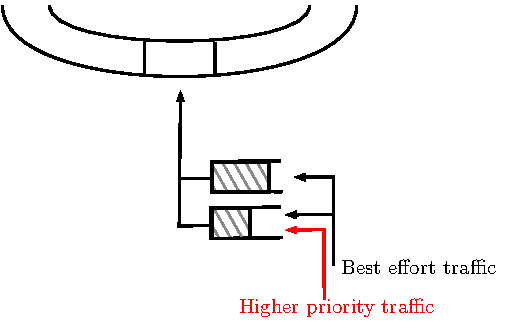
\includegraphics[scale=0.7]{insertion1.pdf}

     \caption{CRAN priorirty mode.}
\end{center}
  \end{figure}
  
 In the next section, one can find the experimental performance evaluation of those two modes which show that, even for the CRAN priority mode, when the network is loaded, the latency of the CRAN messages is not low enough.
 
 Thus, we propose a deterministic approach in which we set the first date at which the antenna starts to emit and then we reserve the slots needed for the CRAN-message by preventing the others node to write in those slots during the previous ring lap of the slot. 
 

  \subsection{Objectives}
    The main challenge of our study is to improve the CRAN-messages latency, such that the process time does not exceed a given time ${\bf T_{max}} $ while not penalizing too much the BE-messages.
    
    To understand the deterministic algorithm, one must introduce the behavior of the antennas.
    \subsection{CRAN message generation}
    The antennas send some heavy packets in the network. First, those packets are carried to the node of the right through an electronic network. Thus, the node is able to transform an electronic packet of $10\mu s$ in an optical packet of $1\mu s$. This multiplexing is explained in (DOC).
    
        \begin{figure}[h!]
\begin{center}   

      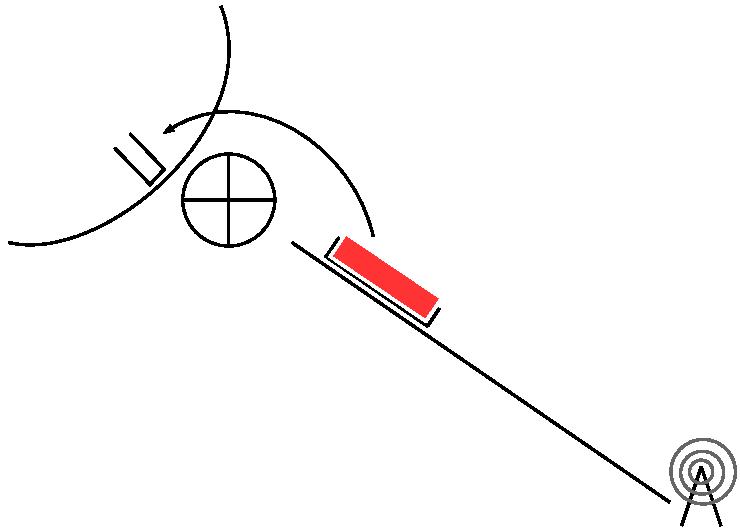
\includegraphics[scale=0.3]{slot1.pdf}
  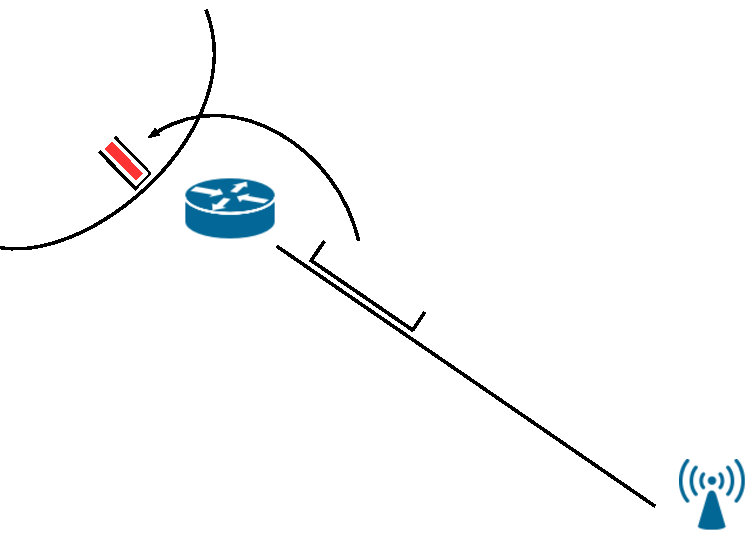
\includegraphics[scale=0.3]{slot2.pdf}
     \caption{Electronic-optical interface.}
     
\end{center}
  \end{figure}
    Thus, an antenna can not send of the ring more than every $10\mu s$. This time is called $EP$ (Emission Period).
    We denote by $ET<P$ (Emission time) the time of the emission of an antenna. Thus, an antenna emits ET/EP packets on the ring, during a period $P$.
    	    
        \begin{figure}[h!]
\begin{center}   

      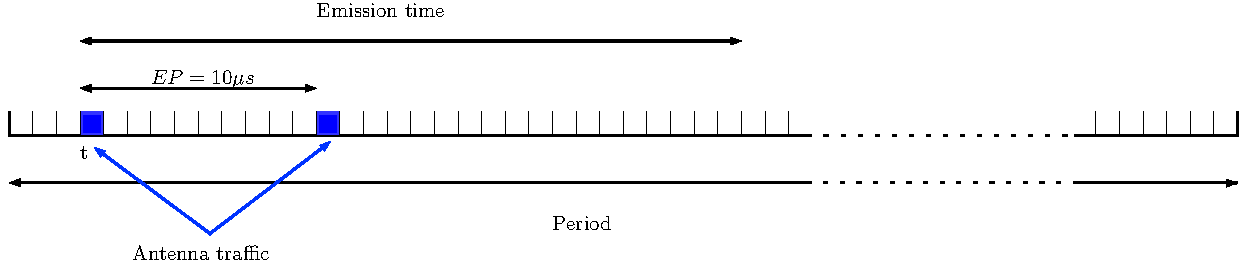
\includegraphics[width=\textwidth]{emission_antenna.pdf}
     \caption{Antenna traffic on the ring.}
  
\end{center}
  \end{figure}
    \subsection{BE message generation}
    	The BE message flow is modeled with a Switch Bernoulli Batch Process (SBBP). Ajouter Doc et details
    
\section{Study of the different insertion policies}

  \subsection{Parameters}
  Peut etre attendre les resultats de youssef pour fixer les deadline et seuil d'envoi dans les simuls.
  \subsection{No management}
  \subsection{CRAN priority}
  Conclure que c'est pas top top, même si c'est clairement mieux en CRAN, et qu'on va faire du determinisme.

\section{Deterministic approach for 0 latency on CRAN}
\label{det}
\subsection{Slot Reservation}
In reservation mode, the main challenge is to reserve the slots for the nodes. Indeed, if a nodes $i$ needs the slot in his wrtting\_slot at time $t$, this slot needs to be reserved at time $t - size\_ring$ by $i$. In this situation, if the slot is already taken by a packet which has been sent by the node $k$, $k$ will remove the packet of the slot during the next lap of the ring, and no other nodes are able to write in this slot before it cames back to the node $i$ a date $t$.

One must study the impact of the reservation on the behavior of the ring. If we want to send a packet in a slot at time $t$, as we described upper, the slot must be reserved one $size\_ring$ before, by the nodes which needs to send the packet. This is the job of the reservation : avoiding others nodes to write in a slot which will be used by the node $i$ at time $t$. Though his reservation allows the CRAN messages to have 0 latency, it impacts the best effort, by avoiding them to use free slots; For the best efforts packets, a slot full represents the same thing as a reserved slot.

Another behavior of a packet on the ring that we must consider is the following one:
 if a node $i$ sends a packet at time $t$, the slot will be used during $t+ size\_ring$ slots. Thus, even if a node emits once, we must take into consideration the fact that the slot is used in the entire ring during $size\_ring$ slots. This means that no others nodes can use this slot to emit a packet on the ring.
This case is problematic if we have $ET =P/2$. For instance, if we want to send a periodic message of size $50$ each $100$ slots on two nodes on a ring, If the node $u$ sends the first packet of it's message at date $0$. Thus, $u$ will emit some packets every periods, during $100$ slots, that is $[kP;ET+kP[, k \in N$. Then, the node $v$ will receive the messages from $u$ each period at time $[kP + \lambda(u,v);ET+kP+\lambda(u,v)[$. Thus, $b$ will emit on the ring at time $[ET + kP + \lambda(u,v);ET+kP+\lambda(u,v) + ET[$, and $a$ will receive those packets from $b$ to $[ET + kP + \lambda(u,v) + \lambda(v,u);ET+kP+\lambda(u,v) + ET + \lambda(v,u)[$, that is $[ET + kP + RS; (k+1)P+RS[$. If we take $k=0$, then $a$ will emit at time $[0;ET[$ then $[P;ET+P[$, and receive the first message of $b$ at time $[ET + RS;  P+RS[$. He one can observe that, during $RS$ slots after $ET$ in $a$, the ring is used by $b$ and then $a$ cannot emit on the ring. Thus, the maximum size that two nodes can share on the ring is $P/2 -RS$.

We distinguish tree cases for the reservation model:
\begin{enumerate}
\item If $2n < EP $.
\item If $2n >EP . \frac{P}{ET+RS}$
\item if $ET = P/2$
\end{enumerate}
	
In the first case, since we have enough frequencies to order the antennas and theirs answers, we only give one block of frequency to each antennas. For instance, if we have $EP = 10$ and $3$ antennas, we give frequencies $0$ and $1$ to the first antenna, $2$ ans $3$ to the second antenna, and $4$ and $5$ to the third antenna.

One can use a smarter method to order k antennas on n frequencies. By expressing $n = q.k + r$, we put a gap of q frequencies between each antennas, except the last r antennas that are spaced by $q+1$ frequencies.

In the second cases, each bloc of $\frac{P}{ET+RS}$ behave like the first case, and we split the different antennas between the different blocks by using the repartition algorithm described above.

In the third case, if $ET = P/2$, we can not schedule the entire emission of a message on the same frequency, because there will be $RS$ slots during while there will be some conflict at the insertion.
Thus, we need to reserve some frequencies to carry the last packet of the messages.
The number of frequencies reserved is $2 .\lceil \frac{2.RS.N}{P}\rceil$.

	

  \subsection{Packing}
  \subsection{Spreading}
  Pour ces deux la, ecrire proprement les ``algos''
  \subsection{Impact on the BE}
  REsultats de simuls
  
  
\section{ Implementation details}

	The source code int C of the simulator used for our experimental results is available on the \href{https://github.com/Mael-Guiraud/Ngreen.git}{ author's github page}.
	\subsection{Initialisation}
	First, we need to put coherent parameters , considering the model. For instance, with the parameters of NGREEN, we can not set more than 10 antennas on the ring. 
	The ring is modeled by a circular table of struct packets. 
	
	\begin{algorithm}[H]
	\MyStruct{packet}{
 		int owner\_id\; \tcp{-1 if there is no packet on the slot.}
  		int size\_CRAN\; \tcp{Nb messages CRAN in the packet\, useful to generate the answers.}
  		int reservation\_id\; \tcp{Useful in the reservation model\, -1 otherwise.}
	}
	\end{algorithm}
	
	For each antenna, we initialize the first date $t$ on which the antenna send some traffic. The antenna will then send a message every 10 slots after $t$, during a fixed total emission time, depending of the throughput of the antenna.


	 In the Insertion Policy models, this date $t$ is randomly drawn with the rand() functions of stdlib. In the Reservation model, this date $t$ is set by the scheduling algorithms described in sec~\ref{det}.
	
	Since the time is discretized, a slot (a unit of time) correspond to one round of a loop. The duration of the loop is set to be large enough to obtain some confident experimental results. During each round of the simulation loop, we first generate the best effort and CRAN traffic, following the laws described in sec~\ref{model}.
	
	Then, we call the \texttt{insert\_packets()} function to send the packets on the ring, if needed (i.e, if some CRAN has been generated, or the BE buffer is large, or old enough).
	Finally, the function \texttt{rotate\_ring()} is called, and every struct packets of the circular ring takes the following position in the table (the last cell of the table take the position 1).
	Afterwards, we call the \texttt{remove\_packets()} function, that free the reading\_slot of a node, if the packet on it has been sent by this node.
	\subsection{BE-Generation}
	The best effort generation follows the SBBP decribed in sec~\ref{model}. Since the batch process have, at the most 10 states, this functions runs in $O(1)$: one random drawing for the transition in the markov chain, another random drawing for the batch process, and the Inverse transform sampling, which is bounded by the number of states.
	\subsection{CRAN-Generation}
	We splitted the CRAN-Generation in two steps. First, the nodes which are not the BBU adds their messages from antennas to buffers, if needed. In a second time, the BBU generates and answer in it's buffer, if there is a CRAN packet in the reading\_slot of the BBU.
	\subsection{Insertion packet}
	A node emits a packet on the ring, in its writting\_slot, if :
\begin{itemize}
\item In no management mode :  if the size of the buffer is greater or equal to $\beta .Q $ ($\beta \in ]0;1] , Q$ is the size of the buffer) , or if the oldest datas has arrived in the buffer before or to $t-\alpha$, ( $t$ is the current slot, and $\alpha$ is the deadline, expressed in slot).
\item In CRAN priority mode : 
	\begin{itemize}
	\item If the BE-buffer satisfy one of the latter condition,
	\item Or if there is some CRAN in the CRAN\_buffer. The packet emitted contains all the CRAN possible, filled with as much BE as possible. 
	\end{itemize}
\item in reservation mode, the slot on the writting\_slot of the node must be not reserved, or reserved for the node. Then the constraints are the same than the CRAN-priority mode.
\end{itemize} 	



\end{document}